% siminos/thesis/chapters/slice.tex
% $Author$ $Date$

% Predrag                           Aug 18 2009
%       extracted from wilczak/blog/flow.tex

\renewcommand{\Group}{\ensuremath{G}}         % Predrag Lie or discrete group

\section{\Slice\ dynamics: Differential formulation}
\label{sec:MovFrameODE}

% Predrag                           Jul 19 2009
% Predrag                           Aug 12 2009

\PublicPrivate{
          }{ % switch to private
The basic idea of the `\mslices' is intuitive and
frequently reinvented, each time under a different name; for example,
it is stated without attribution as the problem 1. of Sect.
6.2 of Arnol'd {\em Ordinary Differential
Equations}\rf{cont:arnold92}. The factorization
\refeq{EquiTraj} is stated on p.~31 of Anosov and
Arnol'd\rf{AnAr88}, who note, without further elaboration,
that in the vicinity of a point which is not fixed by the
group one can reduce the order of a system of differential
equations by the dimension of the group.
For the definition of `slice' see, for example,  Chossat
and Lauterbach\rf{ChossLaut00}. Briefly, a submanifold $\pS_\slicep$
containing $\slicep$ is called a {\em slice} through
$\slicep$ if it is invariant under isotropy
$\Group_\slicep(\pS_\slicep)=\pS_\slicep$. If $\slicep$ is a
fixed point of $\Group$, than slice is invariant under the
whole group. The slice theorem is explained, for example, in
\HREF{http://eom.springer.de/S/s120150.htm} {Encyclopaedia of
Mathematics}.
Slices tend to be discussed in contexts much more difficult
than our application - symplectic groups, sections in absence
of global charts, non-compact Lie groups. We follow
\refrefs{rowley_reconstruction_2000} in referring to a local
group-orbit section as a `slice.' \refRefs{Bredon72,GuiSte90}
and others refer to global group-orbit sections as
`cross-sections,' a term that we would rather avoid, as it
already has a different and well established meaning in
physics. Duistermaat and Kolk\rf{DuiKol00} refer to `slices,'
% on p. 103,
but the usage goes back at least to Guillemin and
Sternberg\rf{GuiSte90} in 1984, Palais\rf{Pal61} in 1961 and
Mastow\rf{Mostow57} in 1957. Bredon\rf{Bredon72} discusses
both cross-sections and slices. Guillemin and
Sternberg\rf{GuiSte90} define the `cross-section,' but
emphasize that finding it is very rare: ``existence of a
global section is a very stringent condition on a group
action. The notion of `slice' is weaker but has a much
broader range of existence.''
    } %end \PublicPrivate{
%%%%%%%%%%%%%%%%%%%%%

In this section we show the connection of symmetry reduction through the
fundamental invariants determined  by a moving frame as in \refsect{sec:mf}
to the \emph{\mframes} introduced in the context of Kahrunen-Lo\'eve
expansion for PDEs by Rowley and Marsden\rf{rowley_reconstruction_2000}.
The basic idea is intuitive and presumably old; for example, it is stated
without attribution as the problem 1. of Sect. 6.2 of Arnol'd
{\em Ordinary Differential Equations}\rf{arnold92}.
 	\PC{the credits have to be totally rewritten -the relevant literature
 is in ChaosBook \\
 we show how {\mframes} is connected with a method for
 symmetry reduction studied in the context of PDEs by Rowley and
 Marsden\rf{rowley_reconstruction_2000}, see also
 \rf{rowley_reduction_2003}, and Beyn and Th\"ummler\rf{BeTh04,Thum05}. }

Consider an $N$-dimensional Lie group $\Group$ acting on $d$-dimensional
space and which, at least locally near $\slicep$, has $N$-dimensional orbits.
The existence of a \slice\ and a moving frame implies that we can
write the full \statesp\
trajectory as $\ssp(t)= \LieEl(t)\,\sspRed(t)$, where the
$(d\!-\!N)$-dimensional \reducedsp\ trajectory $\sspRed(t)$
is on some \slice\, and $\LieEl(t)$ is then the
corresponding curve on the $N$-dimensional group manifold of
the group action that rotates $\sspRed$ into $\ssp$ at time
$t$. The time derivative is then $\dot{\ssp}=
\vel(\LieEl\sspRed) = \dot{\LieEl}\sspRed + \LieEl\velRed$,
where the \reducedsp\ flow field is
$\velRed={d\sspRed}/{dt}$. This leads to
\[
\velRed(\sspRed) = \vel(\sspRed) - \LieEl^{-1} \dot{\LieEl} \, \sspRed
\,,
\]
where we have used the equivariance condition
\refeq{eq:equiv}. The Lie group factor
\[
\LieEl^{-1} \dot{\LieEl} =
\LieEl^{-1}\frac{d~}{dt} e^{\gSpace \cdot \Lg } =
\dot{\gSpace} \cdot \Lg
\]
is the tangent field evaluated at ${\LieEl} = 1$.
Hence the flow in the
$(d\!-\!N)$-dimensional \reducedsp\ is given by:
\beq
\velRed(\sspRed) = \vel(\sspRed) - \dot{\gSpace} \cdot \Lg \, \sspRed
\,,\qquad
\velRed={d\sspRed}/{dt}
\,,
\ee{reducFlow}
for any factorization of the flow of form $\ssp(t)=
\LieEl(t)\sspRed(t)$. To actually integrate these equations
we first have to define the flow factorization by imposing
conditions on $\sspRed(t)$, and then integrate phases
$\gSpace(t)$ on a given \reducedsp\ trajectory $\sspRed(t)$.
We shall demand that the \reducedsp\ is confined to a \slice\
fixed by \refeq{PCsectQ1}.

The time derivative of the slice condition
\refeq{PCsectQ}
\[
\velRed \cdot \sliceTan{a} =
\vel(\sspRed) \cdot \Lg_a \slicep -
\dot{\gSpace}_a (\Lg \sspRed) \cdot \Lg \slicep
= 0
\]
expresses the group phases flow
for the slice fixed by \slicep\ in terms of
\reducedsp\ quantities $\sspRed$, $\vel(\sspRed)$
\beq
\dot{\gSpace}_a = \frac{(\vel \cdot \Lg_a \slicep)}
                       {(\Lg \sspRed) \cdot \Lg \slicep }
\,.
\ee{MFdtheta}
In the pattern recognition and 'template fitting' settings
this is called the ``reconstruction equation''%
\rf{rowley_reconstruction_2000,rowley_reduction_2003}.
The \reducedsp\ flow $d\sspRed/dt = \velRed$
\beq
% \dot{\ssp} =
\velRed = \vel - \frac{(\vel \cdot \Lg_a \slicep )}
                         { (\Lg \sspRed) \cdot \Lg \slicep }
                 \, \Lg_a \sspRed
\,.
\ee{EqMotionMovFramePC}

By construction $\velRed \cdot \Lg
\slicep = 0$, and  the motion stays in the
$(d\!-\!N)$-dimensional \slice. The denominator in
\refeq{MFdtheta} vanishes and the phase velocity
$\dot{\gSpace}(\sspRed)$ diverges whenever the direction of
group action on the \reducedsp\ point is perpendicular to the
direction of group action on the \slice\ point $\slicep$.
Therefore \mslices\ has the same \sset\ as its
post-processing variant, \mframes: the intersection of the slice
with the set of points with group tangent perpendicular to $\sliceTan{}$.

%%%%%%%%%%%%%%%%%%%%%%%%%%%%%%%%%%%%%%%%%%%%%%%%%%%%%%%%%%%%%%%%%%
% computed in vaggelis/testing/flows/CLEfinalTmp.nb
\begin{figure}[ht]
\begin{center}
 (\textit{a})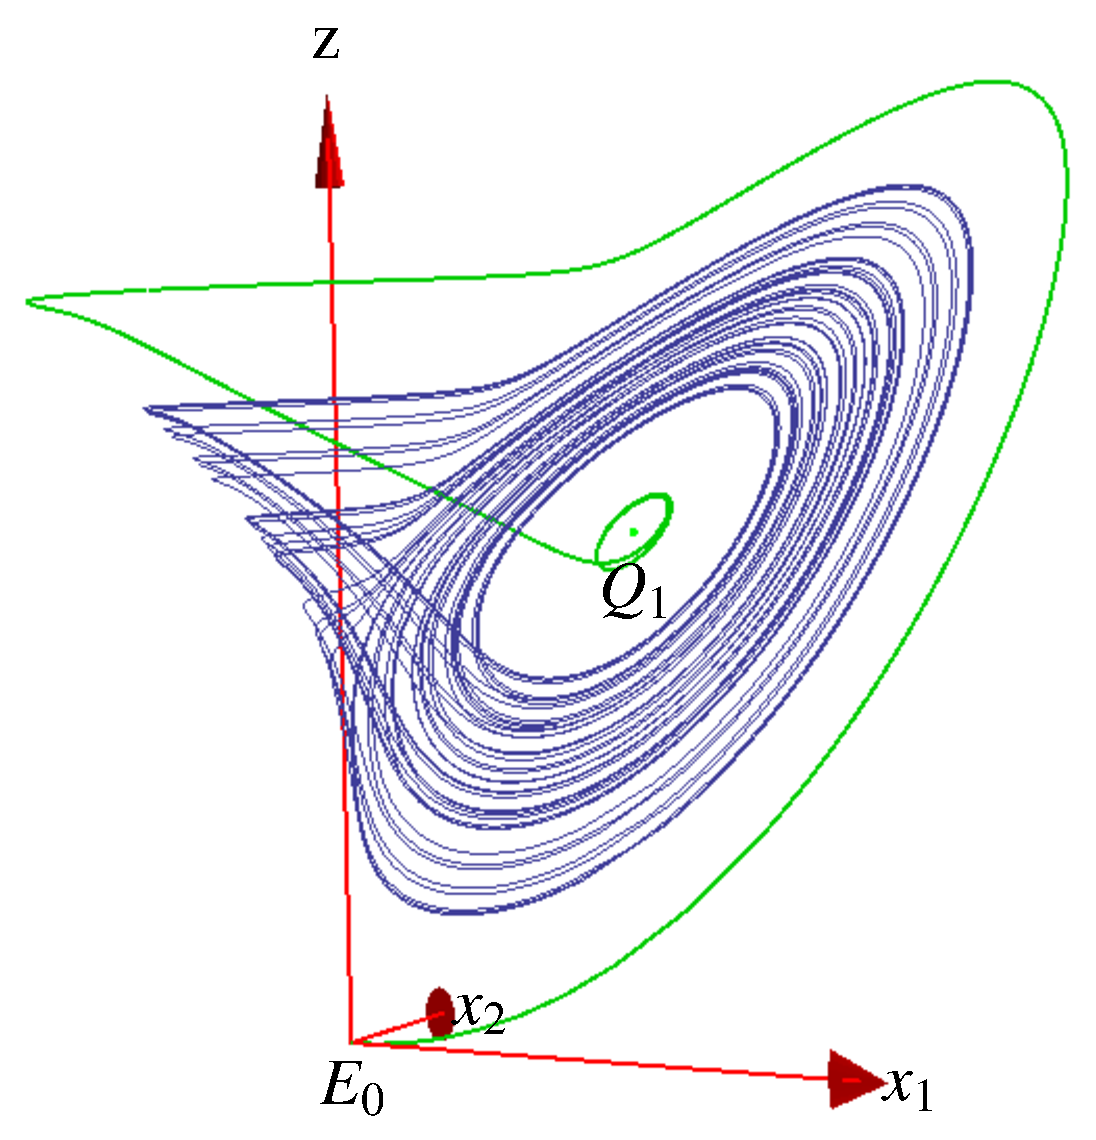
\includegraphics[width=0.43\textwidth]{CLEperpReqb1}
~(\textit{b}) 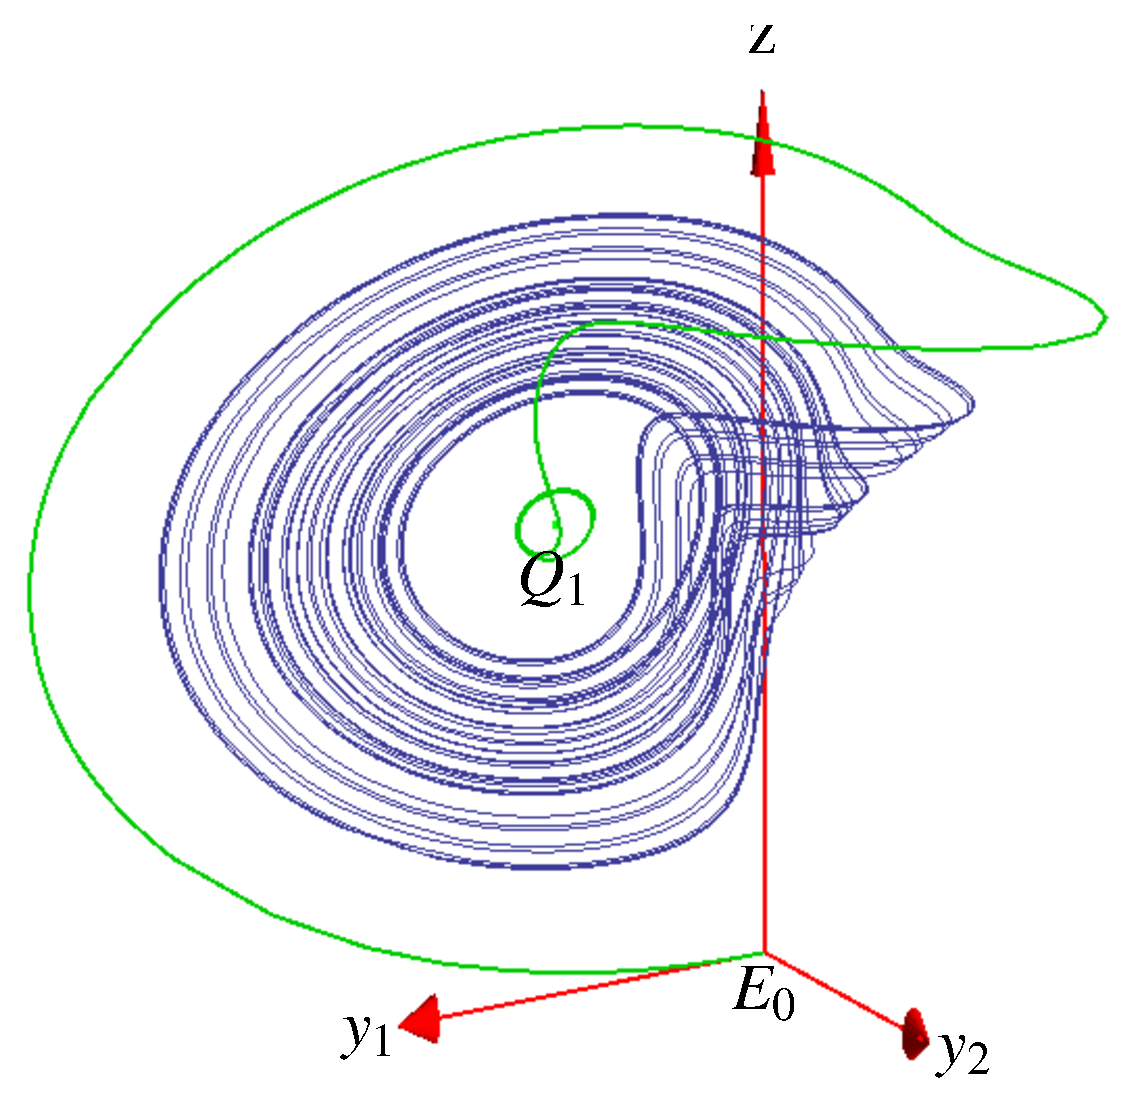
\includegraphics[width=0.43\textwidth]{CLEperpReqb}
\end{center}
\caption{
\Statesp\ portraits of \cLe\ dynamics  in \reducedsp\
obtained by {\Mframes}, \slice\ fixed by a point on the
\reqv\ group orbit, $\slicep  = \ssp_{\REQB{1}}$.
(a) $\{x_1,x_2,z\}$ projection,
(b) $\{y_1,y_2,z\}$ projection.
}
\label{fig:CLEpcSect}
\end{figure}
%%%%%%%%%%%%%%%%%%%%%%%%%%%%%%%%%%%%%%%%%%%%%%%%%%%%%%%%%%%%%%%%
%
A long time trajectory of \refeq{EqMotionMovFramePC} with
$\slicep$ on the \reqv\ \REQB{1} group orbit is shown in
\reffig{fig:CLEpcSect}. Note that this figure is, not coincidentally,
identical to \reffig{fig:CLEmfReqb1}.
As initial condition we chose an initial point on the unstable manifold
of \REQB{1}, rotated back to the \slice\ by angle $\theta$ as
prescribed by \refeq{PCsectQ1}.
    \PC{ in \reffig{fig:CLEpcSect}:\\
        * I think it is a bad idea too plot both $\{x_1,x_2,z\}$ and
          $\{y_1,y_2,z\}$ projections. They are too tightly coupled, and
          look very much the same. That is why in ChaosBook I plot
          $\{x_1,x_2,z\}$ and
          $\{x_1,y_2,z\}$ projections; the latter exhibits the sharp
          singular space discontinuity.
        * Mark $\ssp_{\REQB{}1}$ \\
        * Draw stable eigenvector of $\ssp_{\REQB{}1}$\\
        * State value of $\ssp_{\REQB{}1}$ somewhere
        }

% \PublicPrivate{}{
% % %%%%%%%%%%%%%%%%%%%%%%%%%%%%%%%%%%%%%%%%%%%%%%%%%%
% % % computed by PCunrot.nb
% % \SFIG{PCunrot1}
% % {}{
% % {\Mframes}, continuous time version, for the
% % polar coordinates motivated $x^{*}=(0,1,0,0)$,
% % $x_1=0,\;x_2>0$, \slice. The \CLf\ strange attractor of
% % \reffig{fig:CLE} exhibits a discontinuity at
% % $x_2=0$ in the \reducedsp:
% % $\{x_2,y_2,z\}$ projection.
% % }
% % {fig:PCunrot1}
% % %%%%%%%%%%%%%%%%%%%%%%%%%%%%%%%%%%%%%%%%%%%%%%%%%%
%
% Indeed, the method does encounter singularities in
% subsets of \statesp.
% For example, the \reducedsp\ equations \refeq{PCsectSin}
% for the polar coordinates inspired \slice\
% $x^{*}=(0,1,0,0)$, $x_1=0,\;x_2>0$,
% %this is illustrated by \reffig{fig:PCunrot}.
% %$(\rho_1,\theta_1)$ are polar coordinates, $\rho_1 =
% %\sqrt{\ssp_1^{ 2} + \ssp_2^{2}}$, see \refeq{eq:CartToPol},
% are given by
% \beq
% \dot{\ssp} = \vel - \frac{\vel_1}{\ssp_2} \Lg \cdot \ssp
% \,.
% \ee{EqMotionMovFrame}
% A typical trajectory is shown in \reffig{fig:PCunrot}.
%    \PC{this is not \reffig{fig:PCunrot} - copy correct fig
%        from wilczak/blog
%        }
% }

%\renewcommand{\Group}{\ensuremath{\Gamma}}    % Siminos Lie group
